\section{Code Generation}\label{sec:CodeGen}
The \into tools Overture, OpenModelica and {20-sim} have the ability, to varying degrees, to translate models into platform-independent C source code.
%
Overture can moreover translate VDM models written in the executable subset of VDM++ \cite{Lausdahl&11} (itself a subset of VDM-RT) to Java, but C is the language of interest for the INTO-CPS technology.

The purpose of translating models into source code is twofold.
%
First, the source code can be compiled and wrapped as standalone FMUs for co-simulation, such that the source tool is not required.
%
Second, with the aid of existing C compilers, the automatically generated source code can be compiled for specific hardware targets.

The INTO-CPS approach is to use {20-sim 4C} to compile and deploy the code to hardware targets, since the tool incorporates the requisite knowledge regarding compilers, target configuration \emph{etc.}
%
This is usually done for control software modelled in one of the high-level modelling notations, after validation through the INTO-CPS tool chain.
%
Deployment to target hardware is also used for SiL and HiL validation and prototyping.

For each of the modelling and simulation tools of the INTO-CPS tool chain, code generation is a standalone activity.
%
As such, the reader should refer to the tool-specific documentation referenced in Appendix \ref{appendix:tools} for guidance on code generation.
%
Deliverable D5.1d \cite{INTOCPSD51d} contains the details of how each tool approaches code generation.

The remainder of this section lists information about the code generation capabilities of each tool.
%
Extensive guidance on how to tailor models for problem-free translation to code can be found in the tools' individual user manuals, as referenced in Appendix \ref{appendix:tools}.
%
Further references are given herein.
%
%
%
\subsection{Overture}
Overture provides a code generator for VDM-RT that is geared toward resource-constrained embedded platforms.
%
Of these, PIC32 and ATmega microcontrollers have been tested, as well as Raspberry Pi and typical Intel-based computers.
%
A complete description of Overture's C code generator can be found in Deliverable D5.3d \cite{INTOCPSD5.3d} and in the Overture User Manual, which is accessible through Overture's Help system.
%
As a quick-start guide, this section only provides an introduction to invoking the C code generator, and an overview of the features of VDM-RT that are stable from a code generation point of view.
%
Please note that exporting a source code FMU with Overture (Section \ref{sec:simulators:overture}) automatically invokes the code generator and packages the result as an FMU.

The C code generator is invoked from the context menu in the Project Explorer as shown in Figure \ref{fig:invoking}.
%
%
%
\begin{figure}[ht]
\centering
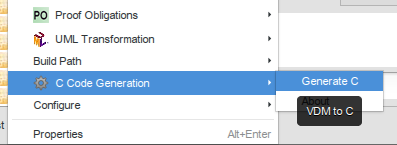
\includegraphics[width=3.2in]{figures/overtureCGInvoking.png}
\caption{Invoking the code generator.}
\label{fig:invoking}
\end{figure}
%
%
%
The code generator currently supports the following VDM-RT language features:
%
%
%
\begin{itemize}
\item  Basic data types and operations:  integers, reals, booleans, \emph{etc.}
%
\item  The \texttt{is\_} type test
%
\item  Quote types
%
\item  Token types
%
\item \texttt{let} expressions
%
\item  Pattern matching (partial support)
%
\item  For and while loops
%
\item \texttt{case} expressions
%
\item  Record types
%
\item  Union types
%
\item  Product types
%
\item  Aggregate types and operations:  sets, sequences and maps
%
\item  Object-oriented features
%
\item  The \texttt{time} expression
%
\item  Pre-condition checks
%
\item  Quantifiers
%
\item  Distributed architectures
\end{itemize}
%
%
%
The following language features are not supported:
%
%
%
\begin{itemize}
\item  Lambda expressions.
%
\item  Post-conditions and invariants.
%
\item  File I/O via the I/O library.
\end{itemize}
%
%
%

A key feature of the C code generator is the use of a garbage collector for memory management.
%
Generating a VDM-RT model to C code via the context menu results in a \texttt{main.c} file containing a skeletal \texttt{main()} function.
%
This function contains calls to \texttt{vdm\_gc\_init()} and \texttt{vdm\_gc\_shutdown()}, the garbage collector initialization and shutdown functions.
%
The collector proper can not be invoked automatically, so calls to the essential function \texttt{vdm\_gc()} must be inserted manually in the main code, for instance after each repetition of a cyclic task.
%
The source code FMU exporter, on the other hand, can handle automatic invocation of the garbage collector, so no manual intervention is required.
%
Please note that it is generally unsafe to insert calls to \texttt{vdm\_gc()} in the generated code.
%
The following is a typical \texttt{main()} function:
%
%
%
%\begin{figure}[ht]
\begin{lstlisting}{language=C}
#include <Vdm.h>

extern void periodic_task();
extern void other_init();
extern void other_shutdown();

extern int keep_going;

int main()
{
	vdm_gc_init();
	other_init();
	
	while(keep_going != 0)
	{
		periodic_task();
		vdm_gc();
	}
	
	vdm_gc_shutdown();
	other_shutdown();
	
	return 0;
}
\end{lstlisting}
%\end{figure}
%
%
%
\subsection{20-sim}\label{ch:codegen:20-sim}
%\revisit{CLP}
{20-sim} supports ANSI-C and C++ code generation through the use of external and user-modifiable code-generation templates.
%
Only a subset of the supported {20-sim} modelling language elements can be exported as ANSI-C or C++ code.
The exact supported features depend on the chosen template and its purpose and are discussed in Section \ref{sec:simulators:20sim}.

The main purpose of the {20-sim} code generator is to export control systems.
Therefore the focus in on running code on limited embedded targets (\emph{e.\@g.\@} Arduino) with no operating system, or as a real-time task on a real-time operating system.
%
The code generated by {20-sim} does not contain any target-related or operating system specific code.
The exported code is generated such that it can be embedded in an external software project.
To run {20-sim} generated code on a target, you can use {20-sim 4C}.
This is a tool that extends the {20-sim} generated code with target code based on target templates \cite{20sim4C}. 

%
%
%
\subsection{OpenModelica}
OpenModelica supports code generation from Modelica to source code targeting both ANSI-C and C++.
From the generated source code, co-simulation and model-exchange FMUs can be built.
The only supported solver in the generated co-simulation FMUs is forward Euler. 
Additional solvers will be supported in the future.
%
%
%
\subsection{RT-Tester/RTT-MBT}
When generating test FMUs from SysML discrete-event state-chart specifications using RTTester/RTT-MBT, the user should be aware of the following sources of errors:
%
%
%
\begin{itemize}
%
\item  Livelock resulting from a transition cycle in the state-chart specification in which all transition guards are true simultaneously.  This can be checked separately using a livelock checker.
%
\item  Race conditions arising from parallel state-charts assigning different values to the same variable.  Model execution in this case will deadlock.
%
\item  State-charts specifying a replacement SUT must be deterministic.
%
\end{itemize}
